\section{Implementation Details}
\label{sec:adaptivity}

In this section, we go over some of the details useful in understanding how the quadtree-adaptive HPS method is implemented. We discuss the patch solver implementation which wraps fast solvers. We provide details related to the mesh library \pforest which is used as a backend for the quadtree data structure.

\subsection{Patch Solvers}
\label{sub:patch_solvers}

When solving \refeq{eq:elliptic_pde} on a single leaf patch, the method used to solve the boundary value problem is called a {\em patch solver} and we denote this function as \texttt{PatchSolver}. The goal of the patch solver is to perform the computations in \refeq{eq:patch_leaf_solve}. The patch solver takes as input the Dirichlet data on the boundary $\textbf{g}_{ext}^{\tau}$, the inhomogeneous data $\textbf{f}^{\tau}$, and some representation of the discretization (i.e., a finite volume grid that corresponds to the patch domain). On output, \texttt{PatchSolver} returns the solution of \refeq{eq:elliptic_pde} on the leaf patch $\textbf{u}^{\tau}$.

Ideally, the patch solver routine takes advantage of fast and optimized solvers for the boundary value problem \refeq{eq:elliptic_pde}. For this implementation, we wrap the FISHPACK routines \citep{swarztrauber1999fishpack} provided in the FISHPACK90 library \citep{adams2016fishpack90}. FISHPACK solves \refeq{eq:elliptic_pde} using a cyclic-reduction method, providing a fast and efficient solver for ``small'' problems. As we use a cell-centered discretization for use with a finite-volume code, we wrap the \texttt{hwscrt} method for our \texttt{PatchSolver}.

\subsection{Building Leaf Level Operators}

At the leaf level, two operators are required: \Stau and \Ttau. The \texttt{PatchSolver} takes the role of \Stau on the leaf. We explicitly compute the matrix \Ttau through use of the patch solver. We define a function \texttt{BuildD2N} that computes \Ttau according to \refeq{eq:map_D2N}. The Dirichlet-to-Neumann matrix depends solely on the discretization -- it is independent of boundary data or inhomogenenous data. Each column of \Ttau is computed column-by-column by solving \refeq{eq:elliptic_pde} with columns of the identity matrix $\textbf{I} \in \real^{4M \times 4M}$ as Dirichlet data \gtau:

\begin{align}
\text{col}_j (\Ttau) = \Ttau \hat{\textbf{e}}_j = \frac{2}{h} (\textbf{I} - \textbf{G} \mathcal{L}_h^{\tau}) \hat{\textbf{e}}_j.
\end{align}

For a constant coefficient elliptic problem, we can take advantage of symmetry in \Ttau to reduce the number of calls to the \texttt{PatchSolver}. This is due to the limited range of the Dirichlet-to-Neumann operator being a boundary operator that depends solely on the discretization of the elliptic problem. To build \Ttau using these optimizations, compute the first $M$ columns of \Ttau and use the following pattern to fill in the remaining blocks:
\begin{align}
\textbf{T}^{\tau} =
\begin{bmatrix}
    \textbf{T}_{w,w} & -\textbf{T}_{w,e} & \textbf{T}_{w,s} & -\textbf{T}_{w,n} \\
    \textbf{T}_{w,e} & -\textbf{T}_{w,w} & \textbf{T}_{w,n} & \textbf{T}_{e,n} \\
    \textbf{T}_{w,s} & -\textbf{T}_{w,n}^T & \textbf{T}_{w,w} & -\textbf{T}_{w,e} \\
    \textbf{T}_{w,n} & \textbf{T}_{w,n}^{'} & \textbf{T}_{w,e} & -\textbf{T}_{w,w} \\
\end{bmatrix}
\end{align}
where $M$ is the size of a leaf patch boundary, and $\textbf{T}_{w,n}^{'}$ is $\textbf{T}_{w,n}$ with reversed columns: $T_{i,j}^{'} = T_{M-i,j}$.

% \begin{align}
%     \Tss{W}{E} &= -\Tss{E}{W} \\
%     \Tss{E}{E} &= -\Tss{W}{W} \\
%     \Tss{S}{E} &= -\Tss{N}{W}^{T} \\
%     \Tss{N}{E} &= -\Tss{E}{W} \\
%     \Tss{W}{S} &= \Tss{S}{W} \\
%     \Tss{E}{S} &= \Tss{N}{W} \\
%     \Tss{S}{S} &= \Tss{W}{W} \\
%     \Tss{N}{S} &= \Tss{E}{W} \\
%     \Tss{W}{N} &= -\Tss{N}{W} \\
%     \Tss{E}{N} &= \Tss{N}{E} \\
%     \Tss{S}{N} &= -\Tss{E}{W} \\
%     \Tss{N}{N} &= -\Tss{W}{W}
% \end{align}

\subsection{Quadtrees and Adaptive Meshes}

As a software library, \pforest provides a quadtree data structure and functions to construct, store, and iterate over leaf-level quadrants in the quadtree.  However, the quadtree-adaptive HPS method requires storage for all nodes in the quadtree; this includes children and parent nodes, not just leaf nodes. This is to store the set of solution operators that act as the matrix factorization of the system matrix. Thus, we require a new data structure that allows for data storage for all nodes in a quadtree. One approach that will later prove to be advantageous for parallel applications is a {\em path-indexed quadtree} \citep{woodward1982explicit,samet1984quadtree}. The path of a node is the unique series of directions required to traverse from the root of the tree to the node. The unique path is encoded as a string containing the sequence of nodes visited.  \reffig{fig:quadtree_indexing} illustrates the path and this unique encoding for a level 3 node.

% \begin{figure}
% \centering
% \begin{tabular}{c c}
% \smallskip
%     \begin{subfigure}[t]{0.8\textwidth}
%         \centering
%         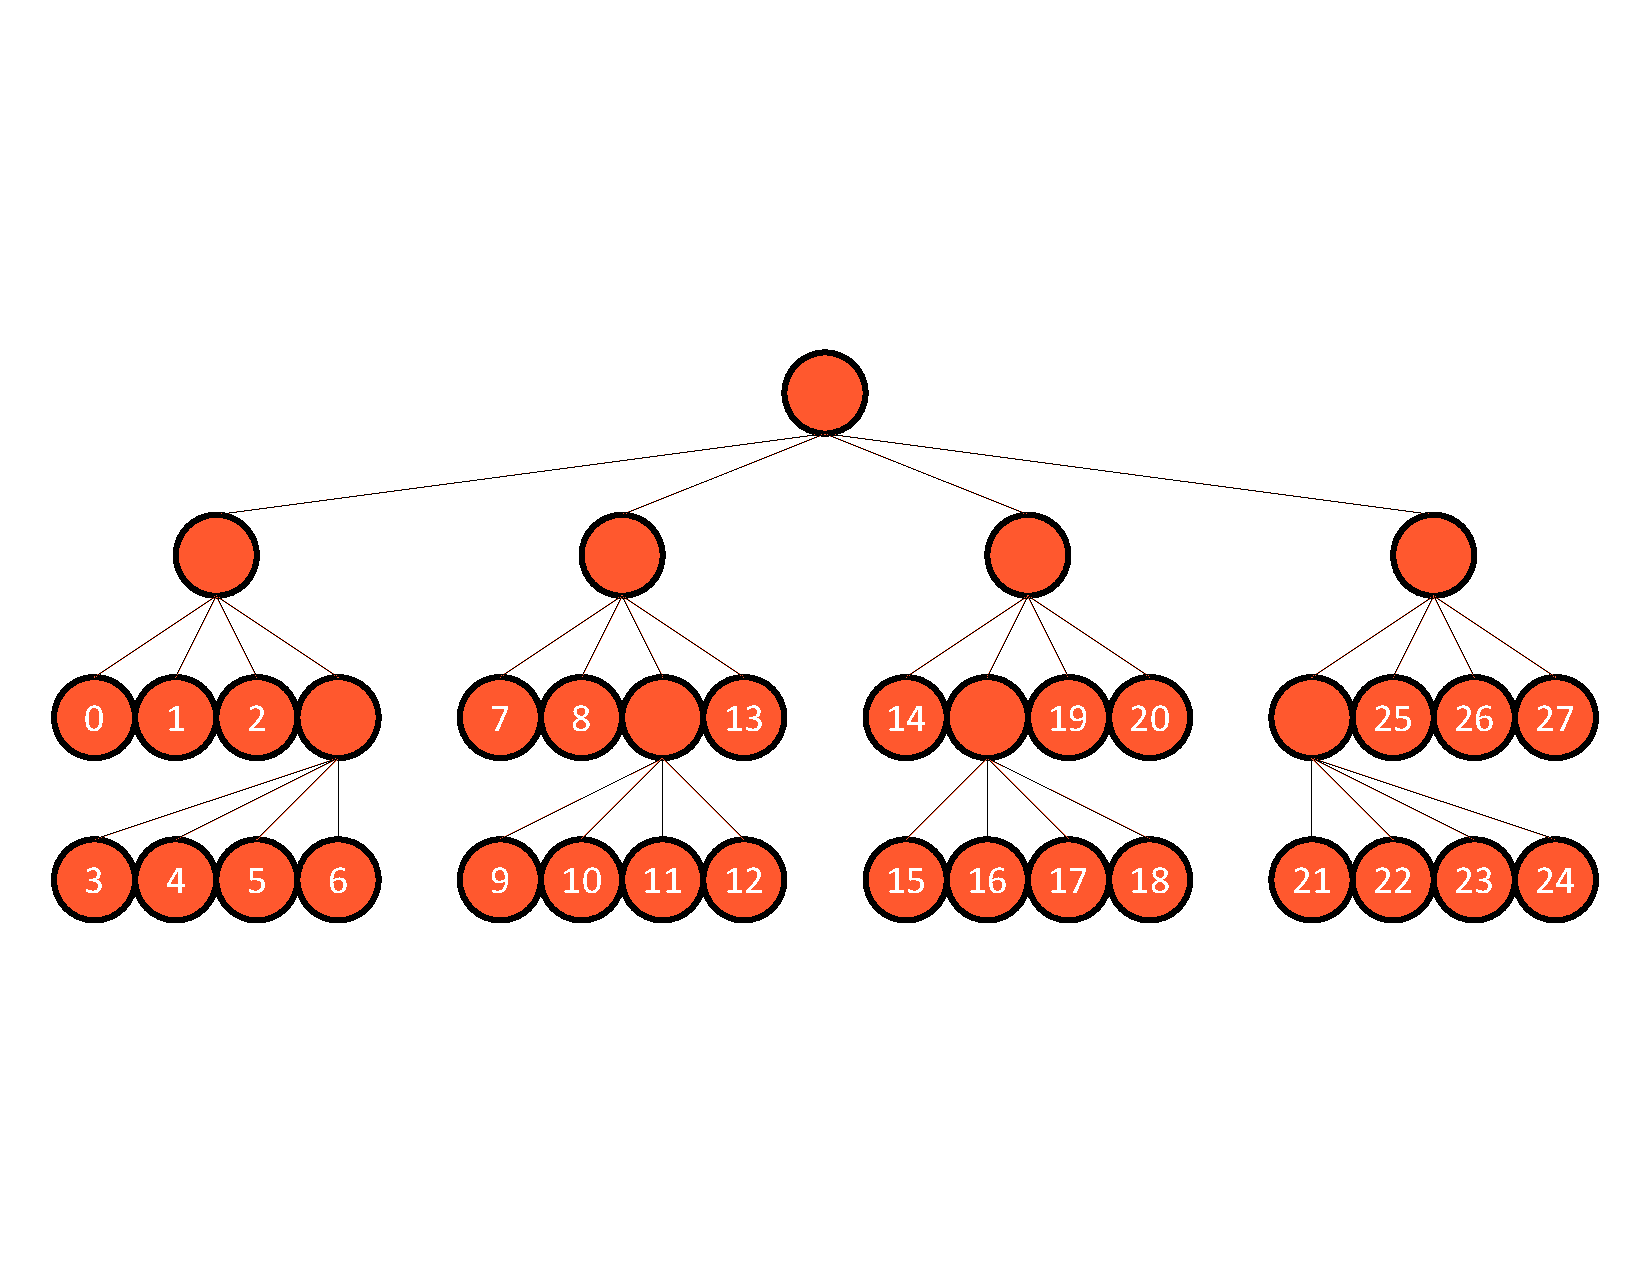
\includegraphics[width=\textwidth, clip=true, trim={0 150 0 150}]{figures/leaf_indexing_tree.pdf}
%         \caption{Leaf-level indexing of quadtree nodes}
%     \end{subfigure}
%     \\
%     \begin{subfigure}[t]{0.8\textwidth}
%         \centering
%         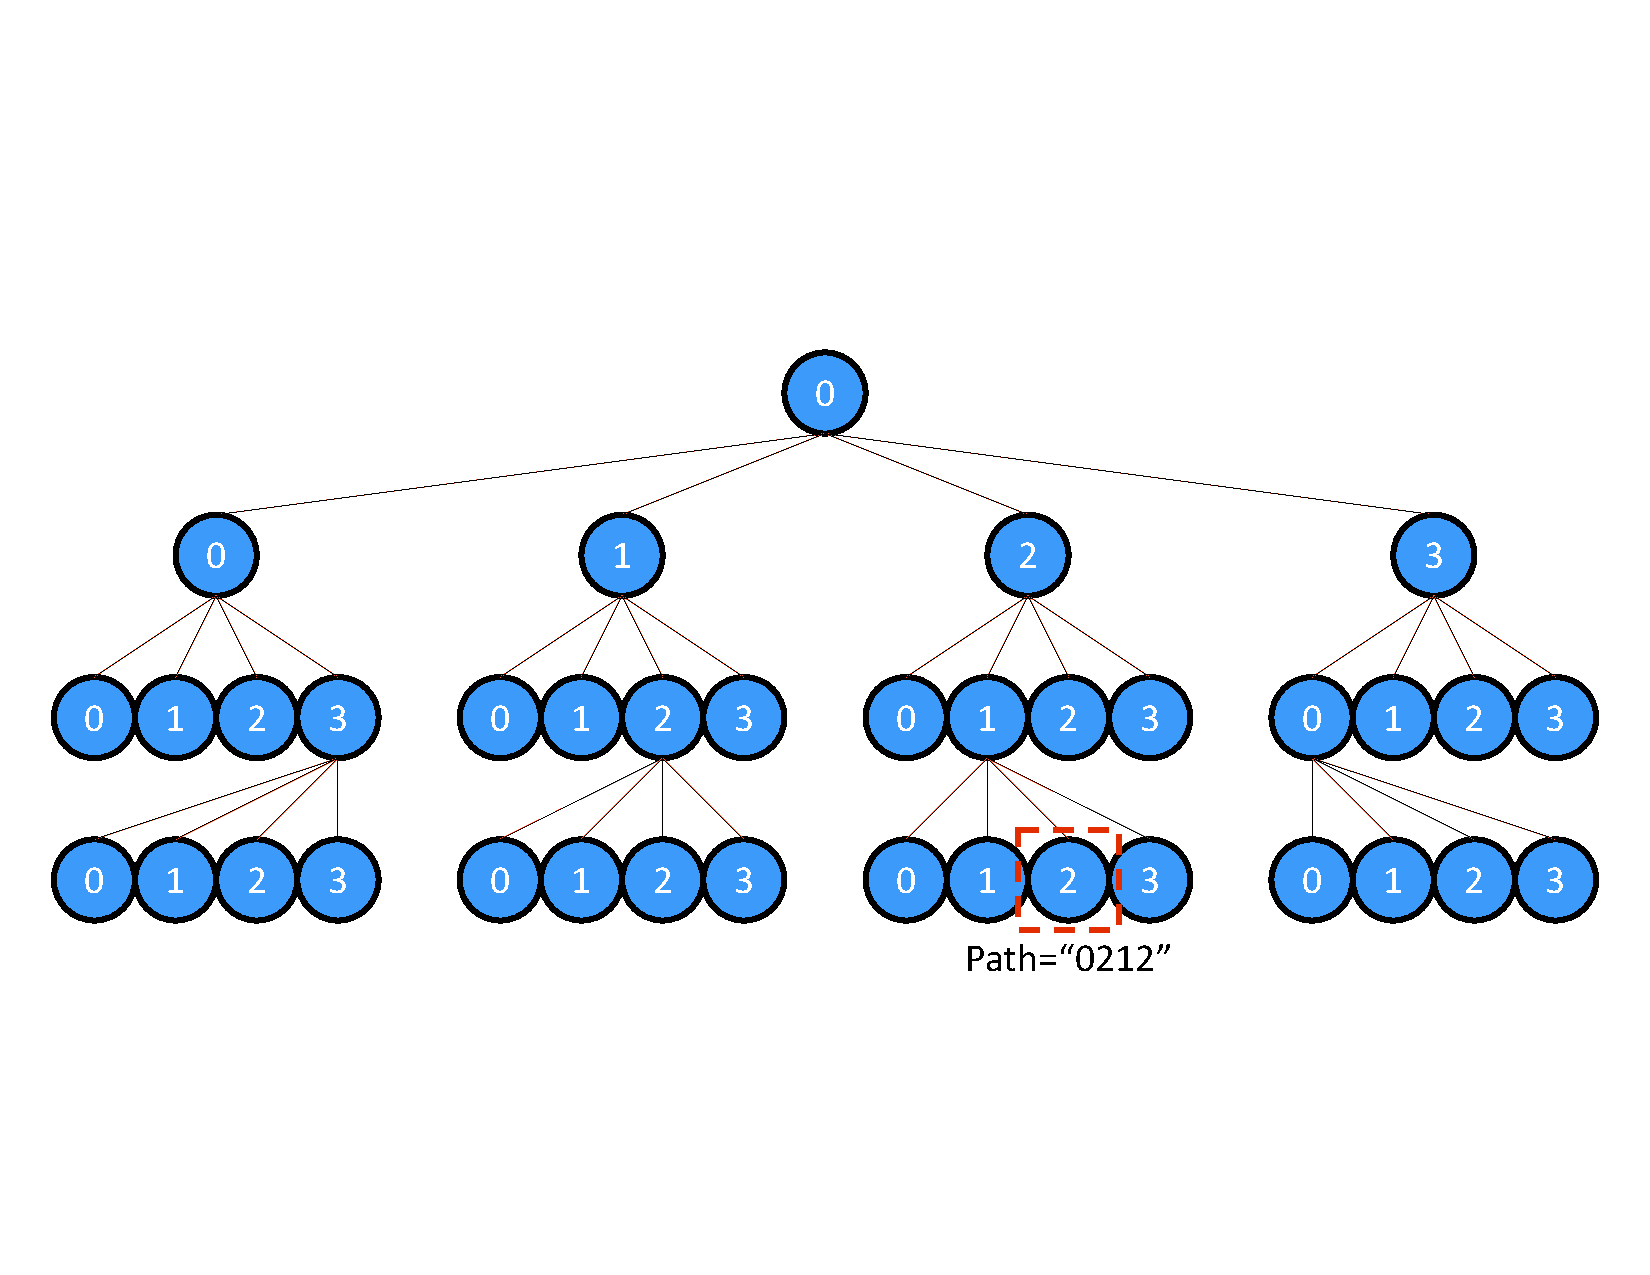
\includegraphics[width=\textwidth, clip=true, trim={0 140 0 150}]{figures/global_indexing_tree.pdf}
%         \caption{Path indexing of quadtree nodes}
%     \end{subfigure}
% \end{tabular}\\
% \caption{Leaf-indexed vs. path-indexed quadtrees. In (a), only the leaves of a quadtree are indexed and stored. In (b), all nodes of the quadtree are indexed and stored according to their unique path.}
% \label{fig:quadtree_indexing}
% \end{figure}

% \begin{figure}
% \centering
% 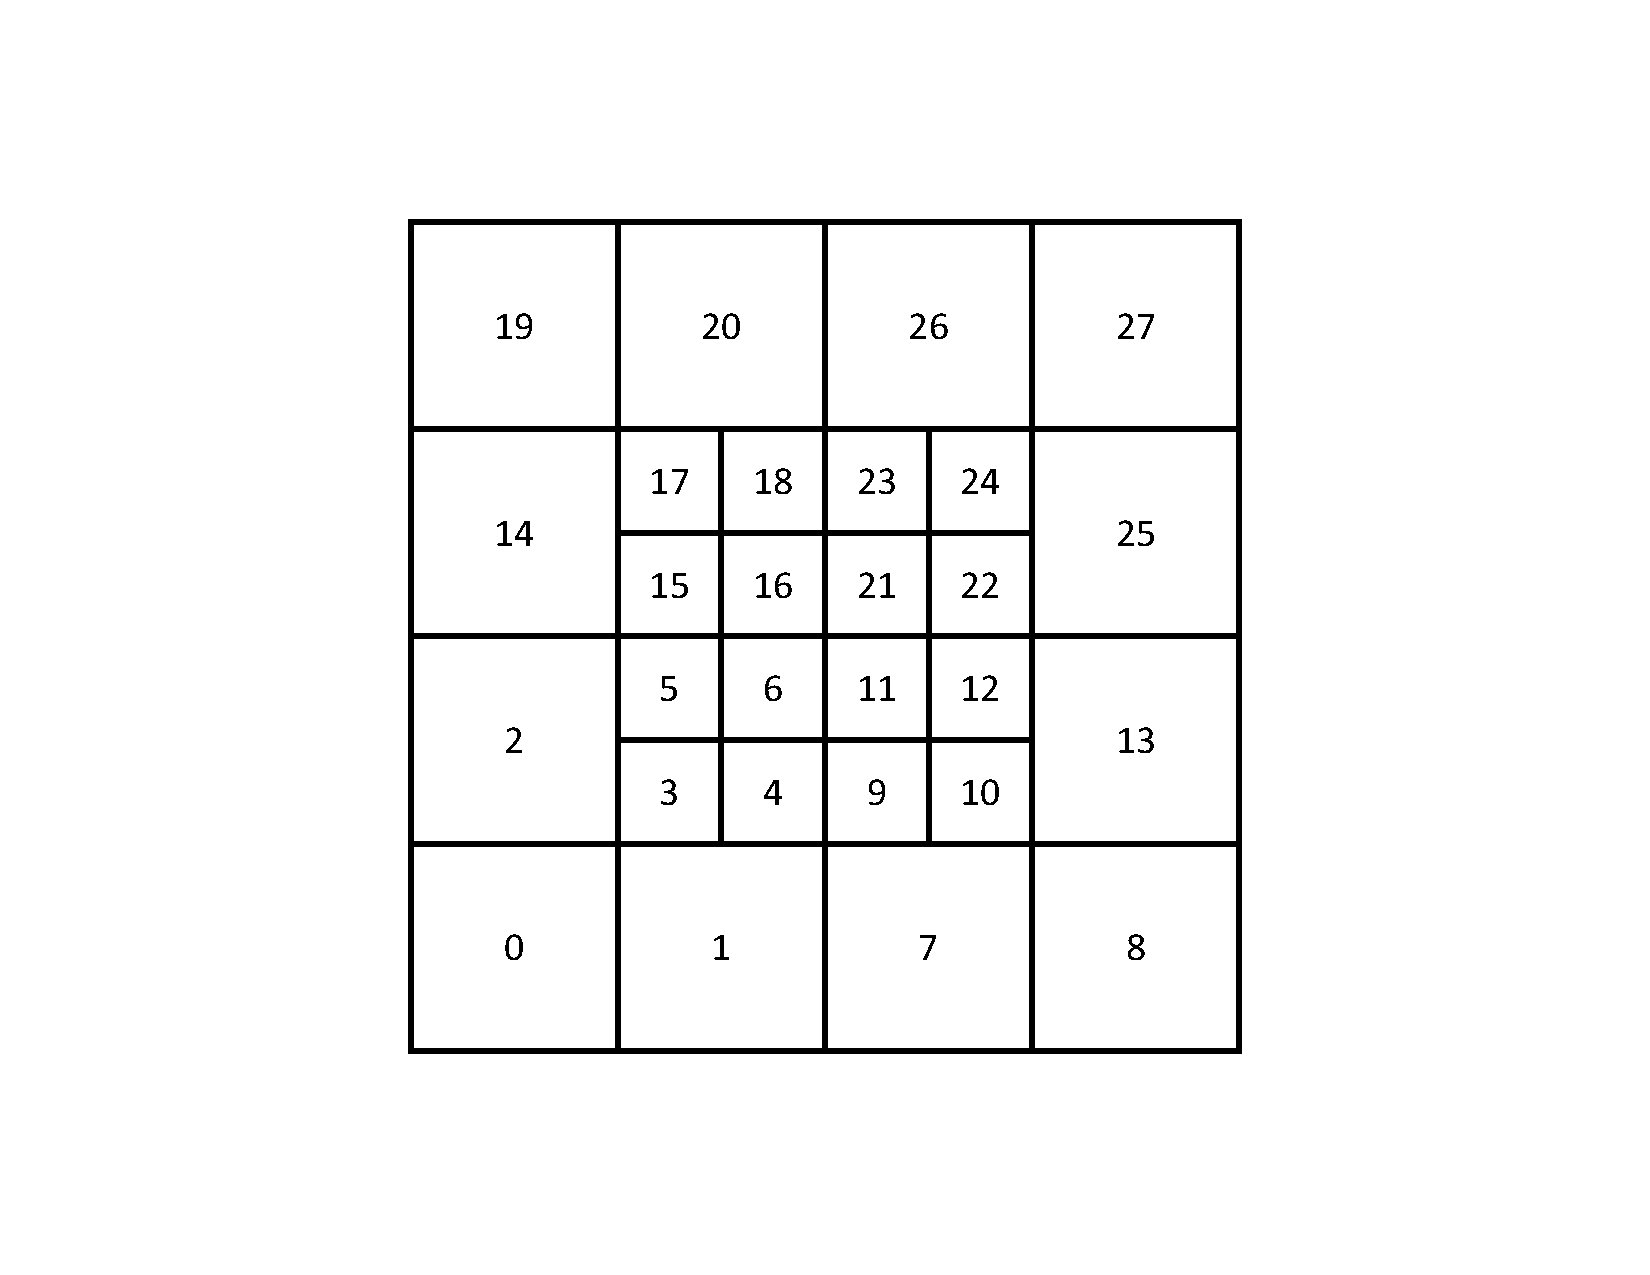
\includegraphics[width=0.4\textwidth]{figures/adaptive_mesh_indexing.pdf}
% \caption{A logically square domain is recursively broken into 4 children domains. This mesh represents refinement criteria that refines the center of the domain. The leaf level nodes are indexed according to a leaf-indexed quadtree and follow a space filling curve.}
% \label{fig:adaptive_mesh}
% \end{figure}

\ignore{As shown in \reffig{fig:quadtree_indexing}, each node in a family can be indexed $0$ to $3$. The highlighted node in \reffig{fig:quadtree_indexing} has a path of $0212$ which corresponds to the steps taken from the root to arrive at that node.}

\ignore{Quadtree data structures, including the path-indexed variety we use here, are not novel. One of the most notable uses of the quadtree data structure was for computer graphics (\citep{woodward1982explicit}, \citep{samet1984quadtree}). A quadtree data structure allows for hierarchical storage at different levels and is a natural application for recursive algorithms. Storing data at all nodes in a quadtree requires knowing the {\em path} of a node. The path of a node is the series of directions taken from the root of the tree to arrive at the particular node. Each node can be uniquely indexed according to the node's path. As shown in \reffig{fig:quadtree_indexing}, each node in a family can be indexed $0$ to $3$. The highlighted node in \reffig{fig:quadtree_indexing} has a path of $0212$ which corresponds to the steps taken from the root to arrive at that node.}

A path-indexed quadtree creates storage for all nodes in the tree through the use of a \texttt{NodeMap}, equivalent to a C++ \texttt{std::map<std::string, Node<T>*>}, where the template parameter \texttt{T} corresponds to a user-provided class to be stored at each node. For the quadtree-adaptive HPS method detailed in this paper, this is a class that holds patch data (grid information, matrices, and vectors). The path is computed by calling \texttt{p4est\_quadrant\_ancestor\_id}. The path-indexed quadtree wraps functions provided by \pforest to construct and iterate over nodes in the path-indexed quadtree.

Two functions provided by {\pforest} allow for a depth-first traversal of a {\pforest} quadtree: \texttt{p4est\_search\_all} and \texttt{p4est\_search\_reorder}. \texttt{p4est\_search\_all} performs a top-down search of the quadtree and provides a callback function with access to a {\pforest} quadrant data structure. This function is used to initialize the path-indexed quadtree by traversing the quadtree in a depth-first order, computing the path for each node, and allocating memory for a \texttt{Node} object in the \texttt{NodeMap}. The function \texttt{p4est\_search\_reorder} also does a top-down search, and provides pre- and post-quadrant callback functions for accessing quadrant data.

Wrapping \texttt{p4est\_search\_reorder}, we define the {\em merge traversal} and the {\em split traversal} of a quadtree. The merge traversal iterates over a quadtree in a post-order fashion, visiting children then parents. When visiting a leaf, a leaf callback is called. When visiting parents, a family callback is used that provides access to the parent and the four children nodes. This is to ``merge'' four children nodes into a parent node, after any leaf data is assigned or computed. The split traversal iterates over a quadtree in a pre-order fashion, with callbacks to families then leaf nodes. This is to provide access to families to ``split'' one parent node into four children nodes. The leaf callback is done last in the split traversal and is used to compute leaf level data once the entire tree has been traversed. The algorithm for the callback function passed to \texttt{p4est\_search\_reorder} is provided in \refalg{alg:quadtree_callback}.

\begin{algorithm}
\caption{\texttt{QuadtreeCallback} Function}
\begin{algorithmic}[0]
    \Require Functions \texttt{LeafCallback}(\texttt{leaf\_node}) \& \texttt{FamilyCallback}(\texttt{parent\_node, children\_nodes})
    \State Compute \texttt{path} from \texttt{p4est\_quadrant\_ancestor\_id}
    \State Let \texttt{node = node\_map[path]}
    \If{\texttt{node} is a leaf} \Comment{Node is a leaf, call leaf callback}
        \State Call \texttt{LeafCallback(node)}
    \Else \Comment{Node is a branch, get children and call family callback}
        \For{i = 0, 1, 2, 3}
            \State \texttt{children\_nodes[i] = map[path + string(i)]}
        \EndFor
        \State Call \texttt{FamilyCallback(node, children\_nodes)}
    \EndIf
\end{algorithmic}
\label{alg:quadtree_callback}
\end{algorithm}

For the quadtree-adaptive HPS method, the leaf callback for the merge traversal is \texttt{BuildD2N}, which solves \refeq{eq:map_D2N} and computes a leaf level Dirichlet-to-Neumann matrix. The family callback wraps the algorithms found in \refsec{sub:4-to-1merge}, which performs the 4-to-1 merge.

The family callback for the split traversal wraps \refeq{eq:solve_eqn}, which applies the solution operator to map parent Dirichlet data to children Dirichlet data (the 1-to-4 split). The leaf callback wraps \texttt{PatchSolver} to solve \refeq{eq:elliptic_pde} on a leaf level using fast solution methods.